\FloatBarrier
\section{Baseline Model Control Condition (Sequential, Heterogeneous Dimensions)\label{res:baseline-control}}
To examine how much of the positive scaling behavior we observed before is due to the model developing expertise within a dimension, rather than developing improving in overall visual processing capacity, we ran the same baseline model on a control version of the benchmark. In this setting, which we term the sequential, heterogeneous dimensions condition, we train the model on permutations of queries from the different dimensions, balancing the number of iterations trained with each ordering of the dimensions. We repeated ninety such iterations, fifteen in each of the six order permutations, and we plot their results in Figure \ref{fig:results-control-sequential-examples-to-criterion} , akin to Figure \ref{fig:results-baseline-sequential-examples-to-criterion}. The overall profile of results appears similar, albeit with less of a ‘hump’ in the second training of the first query, and what appears to be better scaling behavior. We then repeated the catastrophic forgetting plots in Figure \ref{fig:results-control-sequential-first-episode-accuracy}, paralleling Figure \ref{fig:results-baseline-sequential-first-episode-accuracy}. The control model appears to show substantially better forgetting, with the lowest first-epoch accuracy of around 65\%, compared to below 60\% before.

\begin{figure}[!htb]
% \vspace{-0.225in}
\centering
\begin{subfigure}{.49\textwidth}
  \centering
    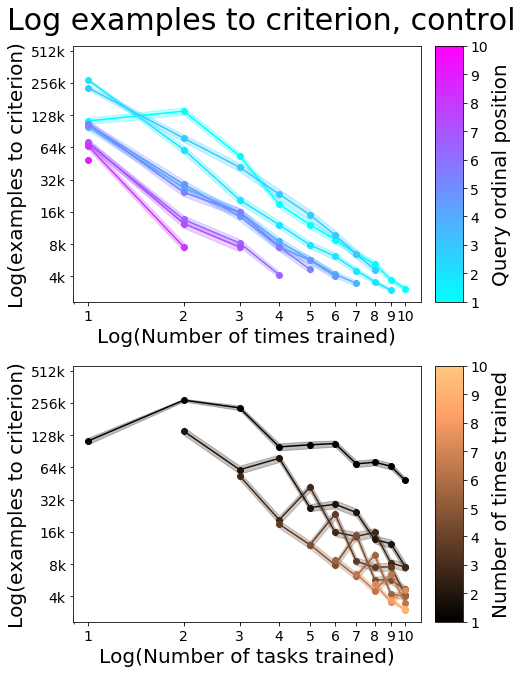
\includegraphics[width=0.85\linewidth]{ch-results/figures/control_sequential/examples_to_criterion.png}
    \caption{ {\bf Log examples to criterion.}}
    \label{fig:results-control-sequential-examples-to-criterion}
\end{subfigure}
\begin{subfigure}{.49\textwidth}
  \centering
    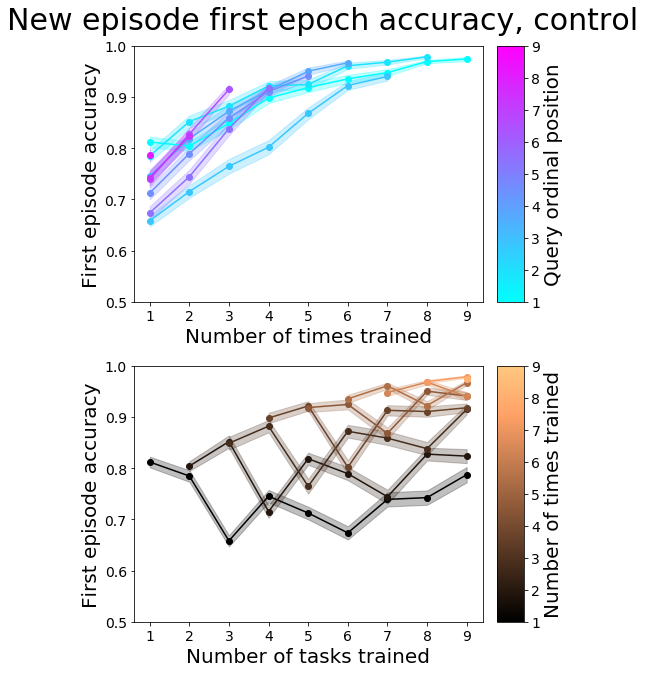
\includegraphics[width=\linewidth]{ch-results/figures/control_sequential/first_episode_accuracy.png}
    \caption{ {\bf New episode first epoch accuracy.}}
    \label{fig:results-control-sequential-first-episode-accuracy}
\end{subfigure}
\caption{{\bf Baseline model control condition results.} This plot depicts the performance of the baseline model on the control condition, following the same format established in Figures \ref{fig:results-baseline-sequential-examples-to-criterion} and \ref{fig:results-baseline-sequential-first-episode-accuracy}.}
\label{fig:results-control-absolute}
\vspace{-0.2in}
\end{figure}

To explicitly compare the conditions Figure \ref{fig:results-control-sequential-comparison-examples-to-criterion} plots the ratio of examples required to reach criterion (which, of course, is the difference in log-examples). We see mixed results with the scaling of the learning behavior: some of the tasks appear to scale better in the homogeneous, baseline condition (points above the $y=1$ line), while others appear to scale better in the control condition (below the line). While the learning scaling behavior results are inconclusive, the catastrophic interference ones are much clearer. Figure \ref{fig:results-control-sequential-comparison-new-episode-accuracy} depicts the difference in new episode first epoch accuracies between these conditions. The control, heterogeneous condition shows lower catastrophic interference at almost every points examined, with more considerable benefits in later tasks in the query order compared to earlier ones.  

\begin{figure}[!htb]
% \vspace{-0.225in}
\centering
\begin{subfigure}{.49\textwidth}
  \centering
    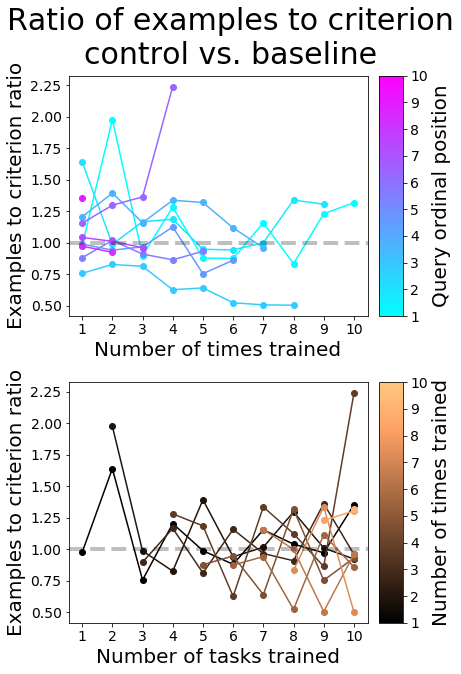
\includegraphics[width=0.85\linewidth]{ch-results/figures/control_sequential/comparison_examples_to_criterion.png}
    \caption{ {\bf Ratio of examples to criterion.}}
    \label{fig:results-control-sequential-comparison-examples-to-criterion}
\end{subfigure}
\begin{subfigure}{.49\textwidth}
  \centering
    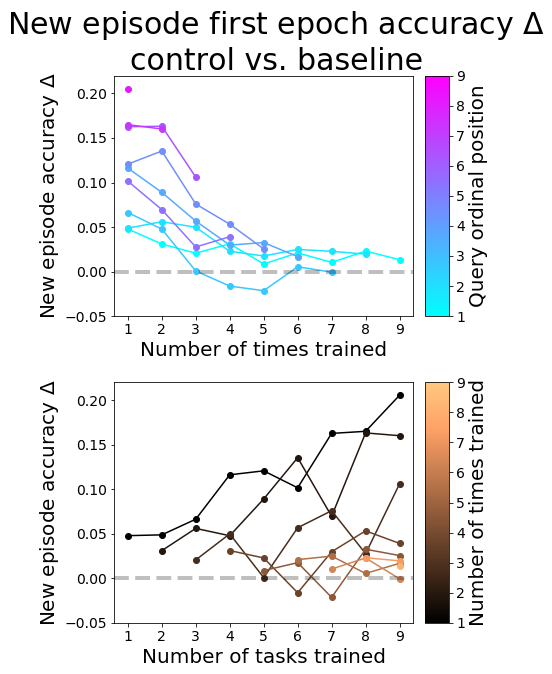
\includegraphics[width=\linewidth]{ch-results/figures/control_sequential/comparison_new_episode_accuracy.png}
    \caption{ {\bf New episode first epoch accuracy difference.}}
    \label{fig:results-control-sequential-comparison-new-episode-accuracy}
\end{subfigure}
\caption{{\bf Baseline model control condition comparison.} \textbf{Left:} Ratio of examples to criterion, regular (homogeneous dimensions) divided by control (heterogeneous dimensions). Points about the $y=1$ line indicate the control condition depicted better performance, and below, the baseline. \textbf{Right:} Difference of new episode first epoch accuracy, subtracting performance on the baseline condition from performance on the control condition. Points above the $y=0$ line indicate lower catastrophic forgetting (and better performance) in the control condition.}
\label{fig:results-control-comparison}
\vspace{-0.2in}
\end{figure}